%!TEX root = ../thesis.tex
\append{Графічний інтерфейс користувача}
\label{appendix: A}

Розробка програмного забезпення включала у себе як імплементацію ітераційних формул переоцінки параметрів моделі, так і розробку графічного інтерфейсу користувача для ефективного керування різними блоками коду. 

Наприклад, на малюнку нижче продемонстровано задання необхідних вхідних даних для генерування відповідного ланцюга Маркова для подальшого розв'язання задачі відновлення елементів множини неявних індексів.

\begin{figure}[H]\centering
    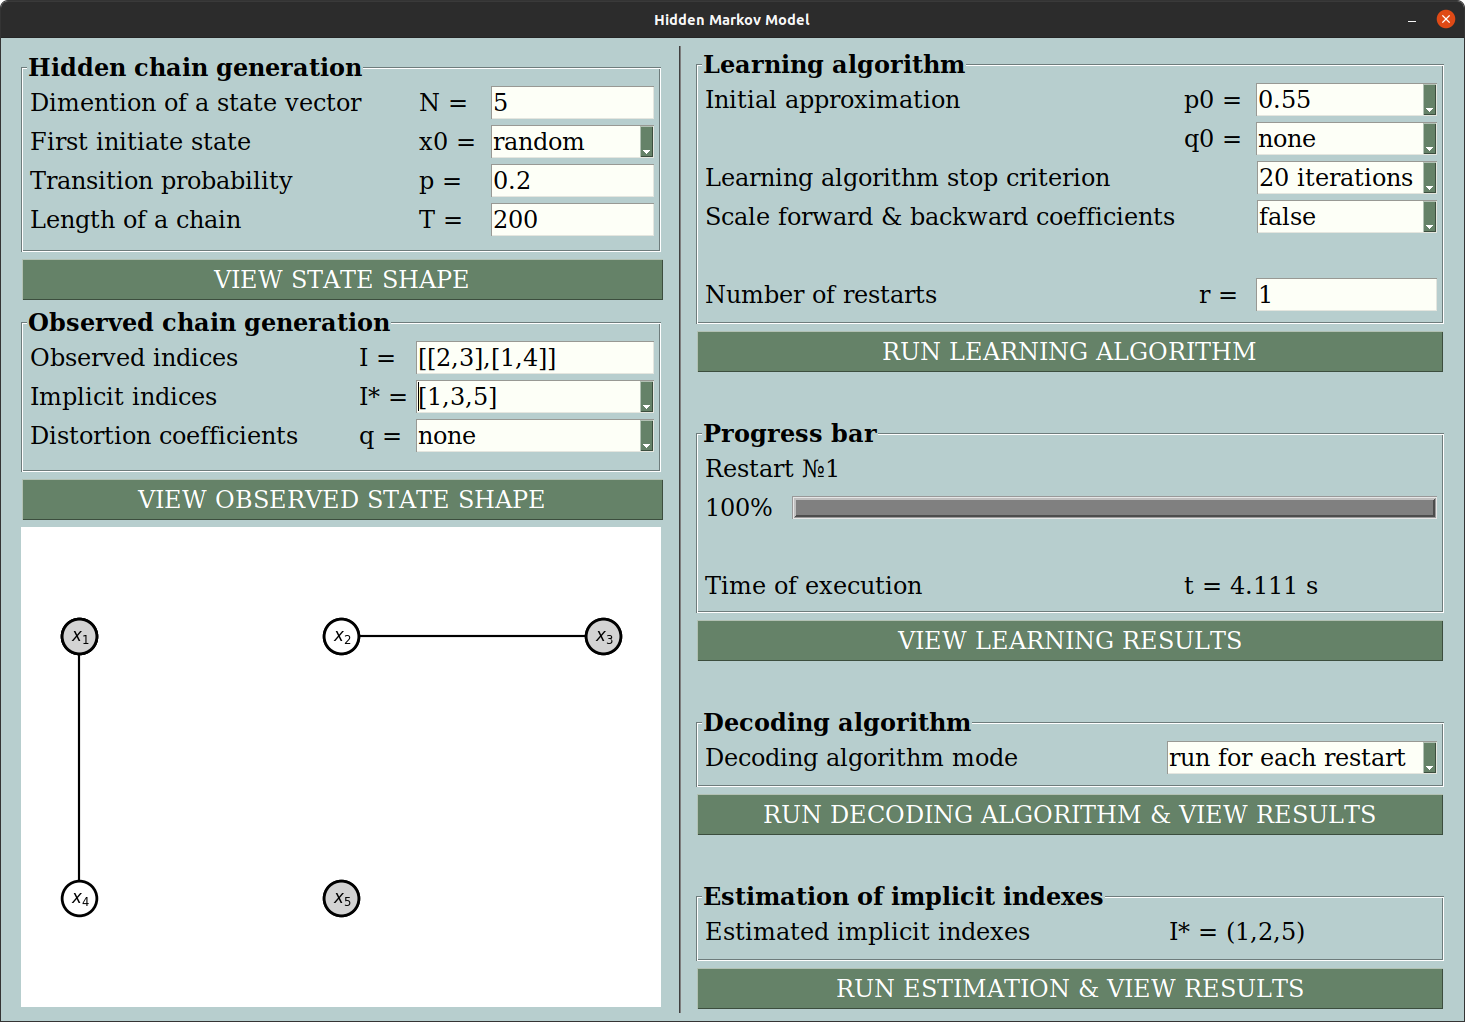
\includegraphics[width=1\linewidth]{Images/GUI.png}
    \caption{Графічний інтерфейс користувача}
    \label{pic: GUI}
\end{figure}

Кожна з відповідних кнопок викликає блоки коду, необхідні для виконання тієї чи іншої задачі. Візуалізація результатів виконується у вигляді наведених у цьому розділі графіків, які демонструються в окремих спливаючих вікнах інтерфейсу.

У лівій нижній частині інтерфейсу схематично зображена конфігурація стану ланцюга: відповідні множини спостережуваних індексів (кожна спостережувана область виокремлюється візуально за з'єднаними ребром вершинами), а також множина неявних індексів, елементи якої позначені сірим кольором.